\begin{slide}
	\begin{block}{Problem}
		Given a planar graph with minimum degree at least $3$, find the length of the smallest circle.
		This value is also called the \emph{girth} of a graph.
	\end{block}
	\pause
	\begin{block}{Solution}
		\begin{itemize}
			\item First, we find a combinatorial embedding.
			\item Simply sort the coordinates of the neighbors of a vertex in ccw order.
			\pause
			\smallskip
			\item We can now traverse the faces of the graph.
			\item We start with an edge, take the head vertex of the edge, find the next edge in cyclic order and continue.
			\pause
			\smallskip
			\item The smallest face we see is the answer.
			\item Runtime: $\mathcal{O}(n\log(n))$ for sorting and $\mathcal{O}(n)$ to enumerate all faces.
			\pause
			\item Verdict: \textcolor{red}{Wrong Answer}\pause?!
		\end{itemize}
	\end{block}
\end{slide}

\begin{slide}
	\centering
	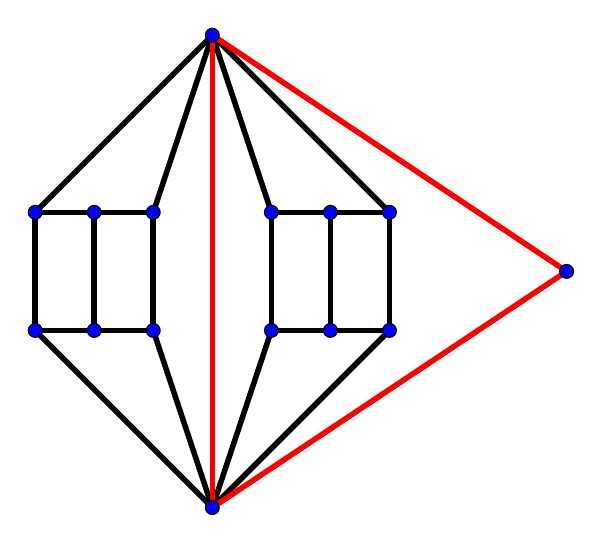
\begin{tikzpicture}[x=0.75cm,y=0.75cm]
		\draw [line width=2.pt] (6.,6.)-- (6.,4.);
		\draw [line width=2.pt] (6.,4.)-- (7.,4.);
		\draw [line width=2.pt] (7.,4.)-- (7.,6.);
		\draw [line width=2.pt] (7.,6.)-- (6.,6.);
		\draw [line width=2.pt] (7.,6.)-- (8.,6.);
		\draw [line width=2.pt] (8.,6.)-- (8.,4.);
		\draw [line width=2.pt] (8.,4.)-- (7.,4.);
		\draw [line width=2.pt] (5.,9.)-- (6.,6.);
		\draw [line width=2.pt] (6.,4.)-- (5.,1.);
		\draw [line width=2.pt] (8.,6.)-- (5.,9.);
		\draw [line width=2.pt] (8.,4.)-- (5.,1.);
		\draw [line width=2.pt] (5.,9.)-- (4.,6.);
		\draw [line width=2.pt] (5.,9.)-- (2.,6.);
		\draw [line width=2.pt] (2.,6.)-- (2.,4.);
		\draw [line width=2.pt] (4.,4.)-- (4.,6.);
		\draw [line width=2.pt] (4.,6.)-- (3.,6.);
		\draw [line width=2.pt] (3.,6.)-- (2.,6.);
		\draw [line width=2.pt] (3.,6.)-- (3.,4.);
		\draw [line width=2.pt] (3.,4.)-- (4.,4.);
		\draw [line width=2.pt] (3.,4.)-- (2.,4.);
		\draw [line width=2.pt] (4.,4.)-- (5.,1.);
		\draw [line width=2.pt] (2.,4.)-- (5.,1.);
		
		\draw [line width=2.pt,color=red] (5.,9.)-- (5.,1.);
		\draw [line width=2.pt,color=red] (5.,1.)-- (11.,5.);
		\draw [line width=2.pt,color=red] (11.,5.)-- (5.,9.);
		
		\draw [fill=blue] (6.,6.) circle (2.5pt);
		\draw [fill=blue] (6.,4.) circle (2.5pt);
		\draw [fill=blue] (7.,4.) circle (2.5pt);
		\draw [fill=blue] (7.,6.) circle (2.5pt);
		\draw [fill=blue] (8.,6.) circle (2.5pt);
		\draw [fill=blue] (8.,4.) circle (2.5pt);
		\draw [fill=blue] (5.,9.) circle (2.5pt);
		\draw [fill=blue] (5.,1.) circle (2.5pt);
		\draw [fill=blue] (11.,5.) circle (2.5pt);
		\draw [fill=blue] (4.,6.) circle (2.5pt);
		\draw [fill=blue] (2.,6.) circle (2.5pt);
		\draw [fill=blue] (2.,4.) circle (2.5pt);
		\draw [fill=blue] (4.,4.) circle (2.5pt);
		\draw [fill=blue] (3.,6.) circle (2.5pt);
		\draw [fill=blue] (3.,4.) circle (2.5pt);
	\end{tikzpicture}
\end{slide}

\begin{slide}
	\begin{block}{Problem}
		Given a planar graph with minimum degree at least $3$, find the smallest circle.
		This property is also called the \emph{girth} of a graph.
	\end{block}
	\begin{block}{Real Solution}
		\pause
		\begin{itemize}
			\item Orient the edges such that each vertex has outdegree $\leq5$ and the graph is a DAG.
			\item Can be done by recursively removing a vertex with degree $\leq5$.
			\pause
			\item Observe that the girth is either $3$, $4$ or $5$.
			\item[$\Rightarrow$] We only need to check if a cycle of length $3$ or $4$ exists.
		\end{itemize}
	\end{block}
\end{slide}

\begin{slide}
	\begin{block}{Problem}
		Given a planar graph with minimum degree at least $3$, find the smallest circle.
		This property is also called the \emph{girth} of a graph.
	\end{block}
	\begin{block}{Real Solution}
		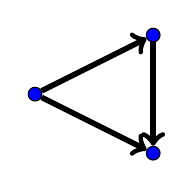
\begin{tikzpicture}[x=0.75cm,y=0.75cm]
			\node[draw,circle,inner sep=1.75pt,fill=blue] (a) at (0,0) {};
			\node[draw,circle,inner sep=1.75pt,fill=blue] (b) at (2,1) {};
			\node[draw,circle,inner sep=1.75pt,fill=blue] (c) at (2,-1) {};
			\draw[->,line width=2pt](a)--(b);
			\draw[->,line width=2pt](a)--(c);
			\draw[->,line width=2pt](b)--(c);
		\end{tikzpicture}
		\hfill
		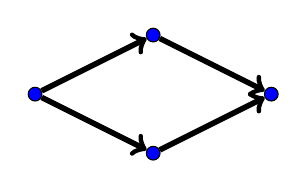
\begin{tikzpicture}[x=0.75cm,y=0.75cm]
			\node[draw,circle,inner sep=1.75pt,fill=blue] (a) at (0,0) {};
			\node[draw,circle,inner sep=1.75pt,fill=blue] (b) at (2,1) {};
			\node[draw,circle,inner sep=1.75pt,fill=blue] (c) at (2,-1) {};
			\node[draw,circle,inner sep=1.75pt,fill=blue] (d) at (4,0) {};
			\draw[->,line width=2pt](a)--(b);
			\draw[->,line width=2pt](a)--(c);
			\draw[->,line width=2pt](b)--(d);
			\draw[->,line width=2pt](c)--(d);
		\end{tikzpicture}
		\hfill
		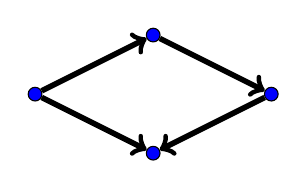
\begin{tikzpicture}[x=0.75cm,y=0.75cm]
			\node[draw,circle,inner sep=1.75pt,fill=blue] (a) at (0,0) {};
			\node[draw,circle,inner sep=1.75pt,fill=blue] (b) at (2,1) {};
			\node[draw,circle,inner sep=1.75pt,fill=blue] (c) at (2,-1) {};
			\node[draw,circle,inner sep=1.75pt,fill=blue] (d) at (4,0) {};
			\draw[->,line width=2pt](a)--(b);
			\draw[->,line width=2pt](a)--(c);
			\draw[->,line width=2pt](b)--(d);
			\draw[<-,line width=2pt](c)--(d);
		\end{tikzpicture}
		\hfill
		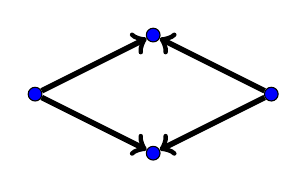
\begin{tikzpicture}[x=0.75cm,y=0.75cm]
			\node[draw,circle,inner sep=1.75pt,fill=blue] (a) at (0,0) {};
			\node[draw,circle,inner sep=1.75pt,fill=blue] (b) at (2,1) {};
			\node[draw,circle,inner sep=1.75pt,fill=blue] (c) at (2,-1) {};
			\node[draw,circle,inner sep=1.75pt,fill=blue] (d) at (4,0) {};
			\draw[->,line width=2pt](a)--(b);
			\draw[->,line width=2pt](a)--(c);
			\draw[<-,line width=2pt](b)--(d);
			\draw[<-,line width=2pt](c)--(d);
		\end{tikzpicture}
		\pause
		\begin{overprint}
			\onslide<2>
			\begin{itemize}
				\item The first three cases can be solved with a limited BFS from each vertex.
				\item We go until depth $3$, so the runtime is $\mathcal{O}(5^3n)$.
			\end{itemize}
			\onslide<3>
			\begin{itemize}
				\item The fourth case can be solved by enumerating all pairs of outgoing edges and checking for duplicates.
				\item We have limited degree, so the runtime is $\mathcal{O}(5^2n\cdot\log(n))$.
			\end{itemize}
		\end{overprint}
	\end{block}
\end{slide}
